\section{Discrete Fourier Transform}
欢迎从连续的、模拟的旧世界,来到离散的、数字的新世界!!!

$f(t)$为连续的Signal,即$t$是一个连续变量:
\begin{enumerate}
	\item 找到一种合理的离散逼近$f(t)$的形式;
	\item 找到一种合理的离散的逼近$f(t)$的Fourier Transform $\mathcal{F}f(s)$的形式;
	\item 找到一种从$f$的离散形式到Fourier Transform $\mathcal{F}f$的离散形式的合理方法。
\end{enumerate}

下面的推导将建立在抽样定理的误用上:
\begin{enumerate}
	\item $f(t)$受限于$0\leq t\leq L$;
	\item $\mathcal{F}f(s)$受限于$0\leq s\leq 2\cdot B$
\end{enumerate}

为什么称之为误用基于两个原因:
\begin{enumerate}
	\item 我们知道Frequency Domain上的带宽是$-B\leq s\leq B$这种形式,但是这里为了方便后面的推导,采用了上方的这种形式。
	\item 实际上这两个假设并不能同时成立,信号不可能同时在时域和频域上都受限。
\end{enumerate}

\subsection{$f(t)$的离散近似}
为了得到一个$f(t)$的离散近似,我们需要在以$\frac{1}{2\cdot B}$为间隔进行采样:
\begin{figure}[H]
	\centering
	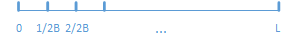
\includegraphics[width=0.4\textwidth]{assets/DFT1.png}
\end{figure}
设$f(t)$内共有$N$个采样点,即:$N\cdot \frac{1}{2\cdot B}=L$,则$N=2\cdot B\cdot N$。

令$t_0=0,t_1=\frac{1}{2\cdot B},\cdots,t_{N-1}=\frac{N-1}{2\cdot B}$。

对$f(t)$进行采样,得:
\begin{align*}
	  & f_{sample}(t)                                      \\
	= & f(t)\cdot \sum\limits_{k=0}^{N-1}\ \sigma(t-t_k)   \\
	= & \sum\limits_{k=0}^{N-1}\ f(t_k)\cdot \sigma(t-t_k)
\end{align*}

采样得到的项分离出$f(t)$的离散近似为:$f(t_0),f(t_1),\cdots,f(t_{N-1})$

但是采样后的$f$仍然是一个连续函数,我们可以对其进行Fourier Transform:
$$
	\mathcal{F}f_{sample}(s)=\sum\limits_{k=0}^{N-1}\ f(t_k)\cdot e^{-2\cdot \pi\cdot i\cdot s\cdot t_k}
$$
\begin{quote}
	就像泰勒级数可以在某一点展开一样,这里只是在$t=t_k$处展开。所以我们说采样后的$f$仍然是一个连续函数。
\end{quote}
\subsection{$\mathcal{F}f(s)$的离散近似}
为了离散化$\mathcal{F}f_{sample}(s)$,我们需要在Frequency Domain进行采样。
\begin{figure}[H]
	\centering
	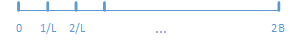
\includegraphics[width=0.4\textwidth]{assets/DFT2.png}
\end{figure}
关于采样,Signal的采样频率是依据该Signal在另一个域的性质决定的。
\begin{enumerate}
	\item 我们在Time Domain采样时依据它在Frequency Domain受限于$[0,2\cdot B]$;
	\item 而在Frequency Domain采样是依据它在Time Domain受限于$[0,L]$,即采样间隔为$\frac{1}{L}$。
\end{enumerate}


设$\mathcal{F}f(s)$上共有$M$个采样点,即:$M\cdot \frac{1}{L}=2\cdot B$,则:$M=2\cdot B\cdot L=N$。我们发现,Time Domain与Frequency Domain上的采样点数目一样多。

令$s_0=0,s_1=\frac{1}{L},\cdots,s_{N-1}=\frac{N-1}{L}$。我们对$\mathcal{F}f_{sample}(s)$进行采样,得:
\begin{align*}
	  & (\mathcal{F}f_{sample})_{sample}(s)                                                                                     \\
	= & \mathcal{F}f_{sample}(s)\cdot \sum\limits_{m=0}^{N-1}\ \delta(s-s_m)                                                    \\
	= & \sum\limits_{k=0}^{N-1}\ f(t_k)\cdot e^{-2\cdot \pi\cdot i\cdot s\cdot t_k}\cdot \sum\limits_{m=0}^{N-1}\ \delta(s-s_m) \\
	= & \sum\limits_{k,m=0}^{N-1}\ f(t_k)\cdot e^{-2\cdot \pi\cdot i\cdot s_m\cdot t_k}\cdot \delta(s-s_m)
\end{align*}

Frequency Domain上的采样值为:
\begin{align*}
	\mathcal{F}f(s_0)     & =\sum\limits_{k=0}^{N-1}\ f(t_k)\cdot e^{-2\cdot \pi\cdot i\cdot s_0\cdot t_k}     \\
	\mathcal{F}f(s_1)     & =\sum\limits_{k=0}^{N-1}\ f(t_k)\cdot e^{-2\cdot \pi\cdot i\cdot s_1\cdot t_k}     \\
	\cdots                                                                                                     \\
	\mathcal{F}f(s_{N-1}) & =\sum\limits_{k=0}^{N-1}\ f(t_k)\cdot e^{-2\cdot \pi\cdot i\cdot s_{N-1}\cdot t_k}
\end{align*}
\subsection{从$f(t)$的离散近似到$\mathcal{F}f(s)$的离散近似}
经过上面两个步骤,$f(t)$被离散化为$f(t_0),f(t_1),\cdots,f(t_{N-1})$;$\mathcal{F}f(s)$被离散化为$\mathcal{F}f(s_0),\mathcal{F}f(s_1),\cdots,\mathcal{F}f(s_{N-1})$。所以我们有:
$$
	\mathcal{F}f(s_m)=\sum\limits_{k=0}^{N-1}\ f(t_k)\cdot e^{-2\cdot \pi\cdot i\cdot s_m\cdot t_k}
$$
其中:
$$
	\begin{cases}
		t_k & = \frac{k}{2\cdot B} \\
		s_m & = \frac{m}{L}
	\end{cases}
$$

令$\underline{f}[k]=f(t_k)$,$\underline{\mathcal{F}f}[m]=\mathcal{F}f(s_m)$。

我们可以知道:
$$
	t_k\cdot s_m=\frac{k\cdot m}{2\cdot B\cdot L}=\frac{k\cdot m}{N}
$$

我们有离散Signal $\underline{f}=(\underline{f}[0],\underline{f}[1],\cdots,\underline{f}[N-1])$,它的Discrete Fourier Transform是离散Signal $\underline{\mathcal{F}f}=(\underline{\mathcal{F}f}[0],\underline{\mathcal{F}f}[1],\cdots,\underline{\mathcal{F}f}[N-1])$则:
\begin{equation}
	\underline{\mathcal{F}f}[m]=\sum\limits_{k=0}^{N-1}\ \underline{f}[k]\cdot e^{-2\cdot \pi\cdot i\cdot \frac{m\cdot k}{N}}
\end{equation}

我们可以把离散Signal看作一个Vector。
\section{对得到的Discrete Fourier Transform公式化简}
\subsection{Time Domain和Frequency Domain的Reciprocity Relationship}
设有一连续Signal在Time Domain与Frequency Domain同时受限,
Time Domain与Frequency Domain都有$N$个采样点(上节课已推导过,Time Domain与Frequency Domain抽样点的数目是一样的),
Time Domain采样间隔为$\Delta t$,Frequency Domain采样间隔为$\Delta s$,
根据不同的$\Delta t$与$\Delta s$可以采集到不同的$\underline{f}$,与$\underline{\mathcal{F}f}$。
\begin{figure}[H]
	\centering
	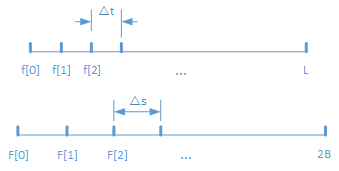
\includegraphics[width=0.4\textwidth]{assets/DFT3.png}
\end{figure}

有$N\cdot\Delta t=L$,$L$为时间上的限制;$N\cdot \Delta s=2\cdot B$,$2\cdot B$为带宽限制:
$$
	\Delta t\cdot \Delta s=\frac{L}{N}\cdot \frac{2\cdot B}{N}=\frac{2\cdot B\cdot L}{N^2}=\frac{N}{N\cdot N}=\frac{1}{N}
$$

Time Domain的采样间隔和Frequency Domain的采样间隔会根据抽样点数成倒数关系(reciprocity relationship)。
这该关系对于进行Discrete Fourier Transform很有现实意义。

当我们确定好Time Domain的采样间隔$\Delta t$与抽样点数$N$时,Frequency Domain的采样间隔$\Delta s$就被固定了,即Frequency Domain分辨率是由Time Domain所做的选择而确定的。
\subsection{引入新符号$\underline{\omega}$}

令$\underline{\omega}$为离散的复指数Signal(或为复指数Vector),且:
\begin{align*}
	\underline{\omega}    & =(1,e^{-2\cdot \pi\cdot i\cdot\frac{1}{N}},e^{-2\cdot \pi\cdot i\cdot\frac{2}{N}},\cdots,e^{-2\cdot \pi\cdot i\cdot\frac{N-1}{N}}) \\
	\underline{\omega}[m] & =e^{-2\cdot \pi\cdot i\cdot\frac{m}{N}}
\end{align*}

那么对$\underline{\omega}$进行幂运算,有:
\begin{align*}
	  & \underline{\omega}^n                                                                                                                                 \\
	= & (1,e^{-2\cdot \pi\cdot i\cdot\frac{n}{N}},e^{-2\cdot \pi\cdot i\cdot\frac{2\cdot n}{N}},\cdots,e^{-2\cdot \pi\cdot i\cdot\frac{(N-1)\cdot n}{N}})    \\
	  & \underline{\omega}^{-n}                                                                                                                              \\
	= & (1,e^{-2\cdot \pi\cdot i\cdot\frac{-n}{N}},e^{-2\cdot \pi\cdot i\cdot\frac{-2\cdot n}{N}},\cdots,e^{-2\cdot \pi\cdot i\cdot\frac{-(N-1)\cdot n}{N}}) \\
	  & \underline{\omega}^{-n}[m] =  e^{-2\cdot \pi\cdot i\cdot\frac{-m\cdot n}{N}}
\end{align*}

把它代入到Discrete Fourier Transform中,则有:
$$
	\underline{\mathcal{F}f}[m]=\sum\limits_{n=0}^{N-1}\ \underline{f}[n]\cdot e^{-2\cdot \pi\cdot i\cdot\frac{m\cdot n}{N}}=\sum\limits_{n=0}^{N-1}\ \underline{f}[n]\cdot \underline{\omega}^{-n}[m]
$$

隐藏序号$m$,有:
\begin{equation}
	\underline{\mathcal{F}f}=\sum\limits_{n=0}^{N-1}\ \underline{f}[n]\cdot \underline{\omega}^{-n}
\end{equation}
\section{Discrete Fourier Transform特性}
\subsection{输入和输出的周期性}
Discrete Fourier Transform的定义迫使我们把输入$\underline{f}$与输出$\underline{\mathcal{F}f}$不仅当作定义在$0$到$N-1$整数上的,并且是周期为$N$的周期离散函数。


\subsection{离散复指数的正交性}
%TODO:在普通的Fourier Transform中的复指数也是有正交性
\begin{align*}
	\underline{\omega}   & =(1,e^{-2\cdot \pi\cdot i\cdot\frac{1}{N}},e^{-2\cdot \pi\cdot i\cdot\frac{2}{N}},\cdots,e^{-2\cdot \pi\cdot i\cdot\frac{N-1}{N}})                 \\
	\underline{\omega}^n & =(1,e^{-2\cdot \pi\cdot i\cdot\frac{n}{N}},e^{-2\cdot \pi\cdot i\cdot\frac{2\cdot n}{N}},\cdots,e^{-2\cdot \pi\cdot i\cdot\frac{(N-1)\cdot n}{N}}) \\
\end{align*}

如果$k\neq l$,则有$\underline{\omega}^k$与$\underline{\omega}^l$是正交的。
这里不把$\underline{\omega}$当作离散Signal,而是把它当作$N$维Vector,我们在讨论Fourier Series复指数的时候引入了正交,这里可谓是它的离散版本,即如果$k\neq l$:
\begin{align*}
	  & \underline{\omega}^k\cdot \underline{\omega}^l                                                                                       \\
	= & \sum\limits_{n=0}^{N-1}\ \underline{\omega}^k[n]\cdot \overline{\underline{\omega}^l[n]}                                             \\
	= & \sum\limits_{n=0}^{N-1}\ e^{2\cdot \pi\cdot i\cdot \frac{k\cdot n}{N}}\cdot \overline{e^{2\cdot \pi\cdot i\cdot \frac{l\cdot n}{N}}} \\
	= & \sum\limits_{n=0}^{N-1}\ e^{2\cdot \pi\cdot i\cdot \frac{k\cdot n}{N}}\cdot e^{-2\cdot \pi\cdot i\cdot \frac{l\cdot n}{N}}           \\
	= & \sum\limits_{n=0}^{N-1}\ (e^{2\cdot \pi\cdot i\cdot \frac{k-l}{N}})^n                                                                \\
	= & \frac{1-(e^{2\cdot \pi\cdot i\cdot \frac{k-l}{N}})^n}{1-e^{2\cdot \pi\cdot i\cdot \frac{k-l}{N}}}                                    \\
	= & \frac{1-e^{2\cdot \pi\cdot i\cdot \frac{k-l}{N}}}{1-e^{2\cdot \pi\cdot i\cdot \frac{k-l}{N}}}                                        \\
	= & \frac{1-[i\cdot\sin(2\cdot\pi\cdot(k-l))+\cos(1\cdot\pi\cdot(k-l))]}{1-e^{2\cdot \pi\cdot i\cdot \frac{k-l}{N}}}                     \\
	= & \frac{1-(0+1)}{1-e^{2\cdot \pi\cdot i\cdot \frac{k-l}{N}}}=0
\end{align*}

如果$k=l$:
\begin{align*}
	  & \underline{\omega}^k\cdot \underline{\omega}^l                                          \\
	= & \sum\limits_{n=0}^{N-1}\ \underline{\omega}^k[n]\cdot\overline{\underline{\omega}^l[n]} \\
	= & \sum\limits_{n=0}^{N-1}\ (e^{2\cdot \pi\cdot i\cdot \frac{k-l}{N}})^n                   \\
	= & \sum\limits_{n=0}^{N-1}\ (e^0)^n\quad (k=l)                                             \\
	= & N
\end{align*}
因此:
\begin{equation}
	\underline{\omega}^k\cdot \underline{\omega}^l=
	\begin{cases}
		0\quad & k\neq l \\
		N\quad & k=l
	\end{cases}
\end{equation}

当$l\neq k$时,$\underline{\omega}^k$与$\underline{\omega}^l$是正交的,但是他们并不是标准正交,因为$\Vert \underline{\omega}^k\Vert=\underline{\omega}^k\cdot \underline{\omega}^k=N$而不是$1$.因此右式为了归一化为标准正交Vector,会把$N$引入到$\underline{\omega}$中。
\section{Inverse Discrete Fourier Transform}
\begin{align*}
	  & \mathcal{F}^{-1}\mathcal{F}f[m]                                                                                                                                                              \\
	= & \frac{1}{N}\cdot \sum\limits_{n=0}^{N-1}\ \underline{\mathcal{F}f}[n]\cdot e^{2\cdot \pi\cdot i\cdot \frac{m\cdot n}{N}}                                                                     \\
	= & \frac{1}{N}\cdot \sum\limits_{n=0}^{N-1}\ (\sum\limits_{n=0}^{N-1}\ \underline{f}[k]\cdot e^{-2\cdot \pi\cdot i\cdot \frac{k\cdot n}{N}})\cdot e^{2\cdot \pi\cdot i\cdot \frac{m\cdot n}{N}} \\
	= & \frac{1}{N}\cdot \sum\limits_{n=0}^{N-1}\ \underline{f}[k]\cdot (\sum\limits_{n=0}^{N-1}\ e^{-2\cdot \pi\cdot i\cdot \frac{k\cdot n}{N}}\cdot e^{2\cdot \pi\cdot i\cdot \frac{m\cdot n}{N}}) \\
	= & \frac{1}{N}\cdot \sum\limits_{n=0}^{N-1}\ \underline{f}[k]\cdot(\underline{\omega}^k\cdot \underline{\omega}^m)                                                                              \\
	= & \frac{1}{N}\cdot \sum\limits_{n=0}^{N-1}\ \underline{f}[k]\cdot N\quad (\underline{\omega}^k\cdot \underline{\omega}^m=\begin{cases}
		0\quad k\neq m \\
		N\quad k=m
	\end{cases})                                           \\
	= & f[m]
\end{align*}

有$\frac{1}{N}$的原因是,离散复指数是正交的,但不是标准正交的。
\section{Discrete Fourier Transform的性质}
\subsection{Discrete Fourier Transform在零点}
$$
	\underline{\mathcal{F}f}(0)=\sum\limits_{n=0}^{N-1}\ \underline{f}[n]\cdot e^{2\cdot \pi\cdot i\cdot \frac{0\cdot n}{N}}=\sum\limits_{n=0}^{N-1}\ \underline{f}[n]
$$

类比到Fourier Transform:
$$
	\mathcal{F}f(0)=\int_{-\infty}^\infty\ f(t)\cdot e^{2\cdot \pi\cdot i\cdot 0\cdot t}\ dt=\int_{-\infty}^\infty\ f(t)\ dt
$$
\subsection{典型离散信号}
\subsubsection{$\underline{1}$}
离散信号$\underline{1}$在各个采样点的采样值都为$1$:
$$\underline{1}=(1,1,\cdots,1)$$
\subsubsection{$\underline{\delta_0}$}
$$\underline{\delta_0}=(1,0,\cdots,0)$$

对其进行Discrete Fourier Transform:
\begin{align*}
	  & \underline{\mathcal{F}}\underline{\delta_0}                                   \\
	= & \sum\limits_{n=0}^{N-1}\ \underline{\delta_0}[n]\cdot \underline{\omega}^{-n} \\
	= & \underline{\delta_0}[0]\cdot \underline{\omega}^0                             \\
	= & 1\cdot \underline{\omega}^0                                                   \\
	= & (1,1,\cdots,1)=\underline{1}
\end{align*}

因此:
\begin{equation}
	\underline{\mathcal{F}}\underline{\delta_0}=\underline{1}
\end{equation}

\subsubsection{$\underline{\delta_k}$}
$$\underline{\delta_k}=(0,0,\cdots,1,0,\cdots,0)$$

对其进行Discrete Fourier Transform:
\begin{align*}
	  & \mathcal{F}\delta_k                                               \\
	= & \sum\limits_{n=0}^{N-1}\ \delta_k[n]\cdot \underline{\omega}^{-n} \\
	= & \underline{\delta_k}[k]\cdot \underline{\omega}^{-k}              \\
	= & 1\cdot \underline{\omega}^{-k}                                    \\
	= & \underline{\omega}^{-k}
\end{align*}
因此:
\begin{equation}
	\underline{\mathcal{F}}\underline{\delta_k}=\underline{\omega}^{-k}
\end{equation}
\subsubsection{$\underline{\omega}^k$}
\begin{align*}
	  & \underline{\mathcal{F}}\underline{\omega}^k[m]                                                                             \\
	= & \sum\limits_{n=0}^{N-1}\ \underline{\omega}^k[n]\cdot \underline{\omega}^{-n}[m]                                           \\
	= & \sum\limits_{n=0}^{N-1}\ e^{2\cdot \pi\cdot i\cdot \frac{k\cdot n}{N}}\cdot e^{-2\cdot \pi\cdot i\cdot \frac{m\cdot n}{N}} \\
	= & \underline{\omega}^k\cdot \underline{\omega}^m                                                                             \\
	= & \begin{cases}
		0 & \ k\neq m \\
		N & \ k=m
	\end{cases}
\end{align*}

因此:
\begin{equation}
	\underline{\mathcal{F}}\underline{\omega}^k=N\cdot \underline{\delta_k}
\end{equation}

\section{Discrete Fourier Transform Matrix}
\subsection{定义}
一般的$\omega$表示为:
$$
	\omega=e^{\frac{-2\cdot\pi}{N}}
$$

Discrete Fourier Transform的变换式可以写成:
$$
	\underline{\mathcal{F}f}[m]=\sum\limits_{n=0}^{N-1}\ \omega^{-m\cdot n}\cdot \underline{f}[n]
$$

其中:
$$
	\omega^{-m\cdot n}=e^{-2\cdot \pi\cdot i\cdot \frac{m\cdot n}{N}}
$$

我们换另外一种表示方式:
$$
	\underline{\omega}^{-n}[m]=e^{-2\cdot\pi\cdot\frac{ n\cdot m}{N}}
$$

上式呈现了一种新的表述,即对离散信号$\underline{f}$进行Discrete Fourier Transform就相当于用$\underline{f}$与酉矩阵$(\omega^-)^{m\cdot n}$相乘:
\begin{align*}
	  & \left[
		\begin{matrix}
			1      & 1               & 1                     & \cdots & 1                     \\
			1      & \omega^{-1}     & \omega^{-2}           & \cdots & \omega^{-(N-1)}       \\
			1      & \omega^{-2}     & \omega^{-4}           & \cdots & \omega^{-2\cdot(N-1)} \\
			\vdots & \vdots          & \vdots                & \vdots & \vdots                \\
			1      & \omega^{-(N-1)} & \omega^{-2\cdot(N-1)} & \cdots & \omega^{-(N-1)^2}     \\
		\end{matrix}
		\right]
	\cdot
	\left[
		\begin{matrix}
			\underline{f}[0]   \\
			\underline{f}[1]   \\
			\underline{f}[2]   \\
			\vdots             \\
			\underline{f}[N-1] \\
		\end{matrix}
		\right]    \\
	= & \left[
		\begin{matrix}
			\underline{\mathcal{F}f}[0]   \\
			\underline{\mathcal{F}f}[1]   \\
			\underline{\mathcal{F}f}[2]   \\
			\vdots                        \\
			\underline{\mathcal{F}f}[N-1] \\
		\end{matrix}
		\right]
\end{align*}

上述式子左边的矩阵就是Discrete Fourier Transform Matrix,Discrete Fourier Transform Matrix是一个$N\times N$的酉矩阵,可以用下面的式子表达:
\begin{equation}
	(\mathcal{F})_{m\cdot n}=\omega^{-m\cdot n}
\end{equation}
\subsection{转置共轭与Inverse Discrete Fourier Transform矩阵}
对Discrete Fourier Transform Matrix  $\mathcal{F}$进行共轭转置,即:
\begin{quote}
	(酉矩阵的逆矩阵与其伴随矩阵相等
	% 复指数的正交性\\
	% 离散复指数的正交性\\
\end{quote}
\begin{align*}
	(\mathcal{F}^{*})_{n\times m} = \overline{(\underline{\mathcal{F}})_{m\times n}} = \overline{\omega^{-m\times n}} = \omega^{m\times n}
\end{align*}

Discrete Fourier Transform矩阵与它的共轭转置矩阵相乘,有:
\begin{align*}
	      & \underline{\mathcal{F}}\cdot \underline{\mathcal{F}}^{*} \\
	=     &
	\left[
		\begin{matrix}
			1      & 1               & 1                & \cdots & 1                 \\
			1      & \omega^{-1}     & \omega^{-2}      & \cdots & \omega^{-(N-1)}   \\
			1      & \omega^{-2}     & \omega^{-4}      & \cdots & \omega^{-2(N-1)}  \\
			\vdots & \vdots          & \vdots           & \cdots & \vdots            \\
			1      & \omega^{-(N-1)} & \omega^{-2(N-1)} & \cdots & \omega^{-(N-1)^2}
		\end{matrix}
		\right]                                                          \\
	\cdot &
	\left[
		\begin{matrix}
			1      & 1              & 1               & \cdots & 1                \\
			1      & \omega^{1}     & \omega^{2}      & \cdots & \omega^{(N-1)}   \\
			1      & \omega^{2}     & \omega^{4}      & \cdots & \omega^{2(N-1)}  \\
			\vdots & \vdots         & \vdots          & \vdots & \vdots           \\
			1      & \omega^{(N-1)} & \omega^{2(N-1)} & \cdots & \omega^{(N-1)^2}
		\end{matrix}
		\right]                                                          \\
	=     & \left[
		\begin{matrix}\underline{\omega}^0\cdot\underline{\omega}^0
			\underline{\omega}^1\cdot\underline{\omega}^0                                                      & \underline{\omega}^2\cdot\underline{\omega}^0     & \cdots & \underline{\omega}^{N-1}\cdot\underline{\omega}^0     \\
			\underline{\omega}^0\cdot\underline{\omega}^1\underline{\omega}^1\cdot\underline{\omega}^1         & \underline{\omega}^2\cdot\underline{\omega}^1     & \cdots & \underline{\omega}^{N-1}\cdot\underline{\omega}^1     \\
			\underline{\omega}^0\cdot\underline{\omega}^2\underline{\omega}^1\cdot\underline{\omega}^2         & \underline{\omega}^2\cdot\underline{\omega}^2     & \cdots & \underline{\omega}^{N-1}\cdot\underline{\omega}^2     \\
			\vdots                                                                                             & \vdots                                            & \vdots & \vdots                                                \\
			\underline{\omega}^0\cdot\underline{\omega}^{N-1}\underline{\omega}^1\cdot\underline{\omega}^{N-1} & \underline{\omega}^2\cdot\underline{\omega}^{N-1} & \cdots & \underline{\omega}^{N-1}\cdot\underline{\omega}^{N-1} \\
		\end{matrix}
		\right]                                                          \\
	=     &
	\left[
		\begin{matrix}
			N      & 0      & 0      & \cdots & 0      \\
			0      & N      & 0      & \cdots & 0      \\
			0      & 0      & N      & \cdots & 0      \\
			\vdots & \vdots & \vdots & \vdots & \vdots \\
			0      & 0      & 0      & \cdots & N
		\end{matrix}
		\right]=N\cdot I
\end{align*}

因此:
\begin{equation}
	\underline{\mathcal{F}}\cdot \underline{\mathcal{F}}^{*}=N\cdot I
\end{equation}

同理:
\begin{equation}
	\underline{\mathcal{F}}^{*}\cdot \underline{\mathcal{F}}=N\cdot I
\end{equation}

通过上面的推导,我们可以可以得到Inverse Discrete Fourier Transform矩阵为:
\begin{equation}
	\underline{\mathcal{F}}^{-1} = \frac{1}{N}\underline{\mathcal{F}}^{*}
\end{equation}

即:
\begin{equation}
	\left( \underline{\mathcal{F}}^{-1} \right)_{m\times n} = \frac{1}{N}\omega^{m\times n}
\end{equation}
这个结果同样也能运用推导Discrete Fourier Transform矩阵的过程得出。

\subsection{运算复杂度}
这里是指矩阵运算中乘法运算的数目,$\underline{\mathcal{F}f}$的每一项运算会花费$N$个乘法运算,其中共有$N$项,即运算复杂度为$N\times N$,用$O(N^2)$表示。

Fast Fourier Transform算法的目的就是为了减少Discrete Fourier Transform的运算复杂度,Fast Fourier Transform的复杂度为$O(NlogN)$。
\section{Discrete Fourier Transform特性}
\subsection{输入与输出离散信号周期性的证明}
Discrete Fourier Transform的输入和输出都具有均具有周期性,周期为$N$。

如果我们把$\omega$表示在复平面上,它在圆上转圈圈:
\begin{figure}[H]
	\centering
	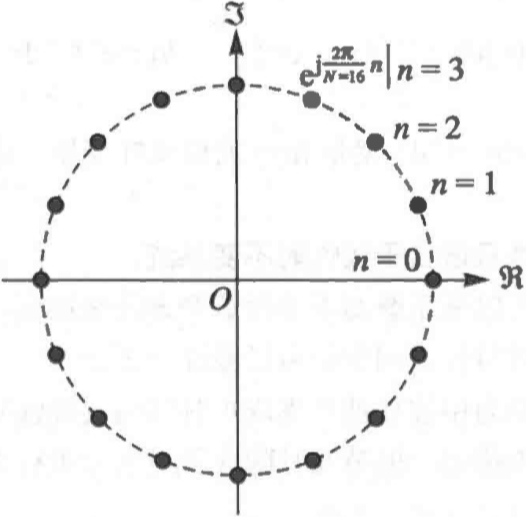
\includegraphics[width=0.4\textwidth]{assets/omega.png}
	\caption{$\omega$的周期性}
\end{figure}

我们取$\underline{\omega}[m] =e^{2\pi i \frac{m}{N}} $。
\subsubsection{Discrete Fourier Transform Matrix中}
\begin{align*}
	  & \underline{\omega}[m+N]               \\
	= & e^{2\pi i\frac{m+N}{N}}               \\
	= & e^{2\pi i\frac{m}{N}}\cdot e^{2\pi i} \\
	= & e^{2\pi i\frac{m}{N}}                 \\
	= & \underline{\omega}[m]                 \\
\end{align*}
同理:
\begin{align*}
	\underline{\omega}^{n}[m]  & = \underline{\omega}^n[m+N]    \\
	\underline{\omega}^{-n}[m] & = \underline{\omega}^{-n}[m+N]
\end{align*}

即$\underline{\omega},\underline{\omega}^n,\underline{\omega}^{-n}$都是周期为$N$的离散复指数信号。


由上述结论推广到Discrete Fourier Transform:
\begin{align*}
	  & \underline{\mathcal{F}f}[m+N]                                \\
	= & \sum_{n=0}^{N-1}\underline{f}[n]\underline{\omega}^{-n}[m+N]
	= \sum_{n=0}^{N-1}\underline{f}[n]\underline{\omega}^{-n}[m]     \\
	= & \underline{\mathcal{F}f}[m]
\end{align*}

因此$\underline{\mathcal{F}f}[m+N] = \underline{\mathcal{F}f}[m]$,表明了对离散信号$\underline{f}$进行Discrete Fourier Transform后会得到周期为$N$的离散信号。

\subsubsection{Inverse Discrete Fourier Transform Matrix}

同理,推广到Inverse Discrete Fourier Transform:
\begin{align*}
	  & \underline{\mathcal{F}}^{-1}\underline{f}[m+N]                                                                                                \\
	= & \frac{1}{N}\sum_{n=0}^{N-1}\underline{f}[n]\underline{\omega}^{n}[m+N]= \frac{1}{N}\sum_{n=0}^{N-1}\underline{f}[n]\underline{\omega}^{-n}[m] \\
	= & \underline{\mathcal{F}}^{-1}\underline{f}[m]
\end{align*}

因此$\underline{\mathcal{F}}^{-1}\underline{f}[m+N] = \underline{\mathcal{F}}^{-1}\underline{f}[m]$,表明了对离散信号$\underline{f}$进行Inverse Discrete Fourier Transform会得到周期为$N$的离散信号。
\subsubsection{总结}
这种周期为$N$的特性是由$\underline{\omega}$的周期性决定的。对某离散信号$\underline{f}$进行Discrete Fourier Transform,会得到周期为$N$的离散信号$\underline{\mathcal{F}f}$,然后对$\underline{\mathcal{F}f}$进行Inverse Discrete Fourier Transform,即$\underline{\mathcal{F}^{-1}\mathcal{F}f}$,也会得到周期为$N$的离散信号$\underline{f}$,这表明了原始信号$\underline{f}$也是周期为$N$的离散信号。

因此有结论如下:进行Discrete Fourier Transform的输入离散信号$\underline{f}$与输出离散信号$\underline{\mathcal{F}f}$都是周期为$N$($N$项)的周期信号;同理进行Inverse Discrete Fourier Transform的输入离散信号$\underline{F}$与输出离散信号$\underline{\mathcal{F}^{-1}\mathcal{F}}$都是周期为$N$($N$项)的周期信号。

% 一开始测量得到的抽样值,必须可以延拓为一系列重复的图像。在离散情况下产生的某些现象,在连续情况下并不存在。原始信号是完全没有周期性的,但是对于有限个测量值的集合情况就不同了。利用Fourier Transform分析,必须使信号具有周期性。在信号没有显示出周期性的情况下,变换会产生周期性。

\subsection{索引的独立性}
周期性可以说是限制,因为我们需要用周期信号来看待将被进行Decrete Fourier Transform、IDecrete Fourier Transform的离散信号,但是这个特性也带来了简单有益的结论:索引的独立性(independence of indexing)。

由于$\underline{f}$与$\underline{\omega}$都具有周期性,因此在计算Decrete Fourier Transform时可以采用任意连续$N$个采样,即:

\begin{align*}
	\underline{\mathcal{F}f} =  \sum_{n=0}^{N-1}\underline{f}[n]\underline{\omega}^{-n} = \sum_{n=1}^{N}\underline{f}[n]\underline{\omega}^{-n}
\end{align*}

我们也可以把零点放置取样值的中间,即:
\begin{align*}
	\underline{\mathcal{F}f} =  \sum_{n=-\frac{N-1}{2}}^{\frac{N-1}{2}}\underline{f}[n]\underline{\omega}^{-n}
\end{align*}

当$N$为奇数时:
\begin{align*}
	\underline{\mathcal{F}f} = \sum_{n=-\frac{N-1}{2}}^{\frac{N-1}{2}}\underline{f}[n]\underline{\omega}^{-n}
\end{align*}

当$N$为偶数时:
\begin{align*}
	\underline{\mathcal{F}f} =  \sum_{n=-\frac{N}{2}+1}^{\frac{N}{2}}\underline{f}[n]\underline{\omega}^{-n}
\end{align*}

在连续的情况下,我们总是考虑对称性,但是在离散的情况下,我们对对称性就没有那么看重了,我们看重的是周期性。
\subsection{离散信号的反转及其Decrete Fourier Transform的对偶性}
\subsubsection{离散信号反转的定义}
在讨论连续信号的反转的时候,连续信号$f(x)$的反转为$f^-(x) = f(-x)$,而这里离散信号的反转被定义为$\underline{f}^{-}[m] = \underline{f}[-m]$,也就是说,如果有离散信号:
\begin{align*}
	\underline{f} = \left(\underline{f}[0],\underline{f}[1],\underline{f}[2],\cdots,\underline{f}[N-1] \right)
\end{align*}

它的反转为:
\begin{align*}
	\underline{f}^- = \left( \underline{f}[0],\underline{f}[-1],\underline{f}[-2], \cdots ,\underline{f}[-(N-1)] \right)
\end{align*}

离散复指数$\underline{\omega}$的反转为:
\begin{align*}
	\underline{\omega}^- = \left( 1,e^{-2\pi i\frac{1}{N}},e^{-2\pi i\frac{2}{N}},\cdots,e^{-2\pi i\frac{N-1}{N}} \right) = \underline{\omega}^{-1}
\end{align*}

同理有:
\begin{align*}
	\left(\underline{\omega}^n \right)^-    & = \underline{\omega}^{-n} \\
	\left(\underline{\omega}^{-n} \right)^- & = \underline{\omega}^{n}
\end{align*}
\subsubsection{Decrete Fourier Transform对偶性讨论}
对离散信号$\underline{f}$的反转$\underline{f}^-$进行Decrete Fourier Transform:
\begin{align*}
	  & \underline{\mathcal{F}f}^-                                                                                \\
	= & \sum_{n=0}^{N-1}\underline{f}^-[n]\underline{\omega}^{-n}                                                 \\
	= & \sum_{n=0}^{N-1}\underline{f}[-n]\underline{\omega}^{-n}    \quad (definition\ of\ reversed\ signal)      \\
	= & \sum_{n=0}^{N-1}\underline{f}[N-n]\underline{\omega}^{-n}   \quad (\underline{f}\ is\ period\ of\ N)      \\
	= & \sum_{l=N}^1\underline{f}[l]\underline{\omega}^{l-N}        \quad (letting\ l=N-n)                        \\
	= & \sum_{l=N}^1\underline{f}[l]\underline{\omega}^l            \quad (\underline{\omega}\ is\ period\ of\ N) \\
	= & \sum_{l=0}^{N-1}\underline{f}[l]\underline{\omega}^l        \quad (independence\ of\ indexing)            \\
	= & \sum_{l=0}^{N-1}\underline{f}[l](\underline{\omega}^{-l})^-                                               \\
	= & \left(
	\sum_{l=0}^{N-1}\underline{f}[l]\underline{\omega}^{-l} \right )^-                                            \\
	= & \left(\underline{\mathcal{F}f}\right )^-
\end{align*}

因此:
\begin{equation}
	\underline{\mathcal{F}f}^- = \left( \underline{\mathcal{F}f} \right)^-
\end{equation}

对离散信号连续进行两次Decrete Fourier Transform:
\begin{align*}
	  & \underline{\mathcal{F}}\underline{\mathcal{F}f}                                                                                                                                                             \\
	= & \sum_{k=0}^{N-1}\left(\sum_{n=0}^{N-1}\underline{f}[n]\underline{\omega}^{-n}[k]\right)\underline{\omega}^{-k}                                                                                              \\
	= & \sum_{n=0}^{N-1}\underline{f}[n]\left(\sum_{k=0}^{N-1}\underline{\omega}^{-n}[k]\underline{\omega}^{-k}\right)                                                                                              \\
	= & \sum_{n=0}^{N-1}\underline{f}[n]\left(\underline{\mathcal{F}}\underline{\omega}^{-n}\right)                                                                                                                 \\
	= & \sum_{n=0}^{N-1}\underline{f}[n]\cdot N\underline{\delta_{-n}}                                                                                                                                              \\
	= & N\sum_{n=0}^{N-1}\underline{f}[n]\underline{\delta_{-n}}                                                                                                                                                    \\
	= & N\sum_{n=0}^{N-1}\underline{f}[n]\left(\underline{\delta_n}\right)^-                                                                                                                                        \\
	= & N\left(\sum_{n=0}^{N-1}\underline{f}[n]\underline{\delta_n}\right)^-\qquad\left(\sum_{n=0}^{N-1}\underline{f}[n](\underline{\delta_n})^-[m]=\sum_{n=0}^{N-1}\underline{f}[n]\underline{\delta_n}[-m]\right) \\
	= & N\left(\sum_{n=0}^{N-1}\underline{f}[n]\underline{\delta_n}[0],\sum_{n=0}^{N-1}\underline{f}[n]\underline{\delta_n}[1],\cdots,\sum_{n=0}^{N-1}\underline{f}[n]\underline{\delta_n}[N-1]\right)^-
\end{align*}

我们来分析一下$\sum_{n=0}^{N-1}\underline{f}[n]\underline{\delta_n}[0]$,其中:
$$
	\underline{\delta_n}[m]=\begin{cases} 1 & \quad m=n     \\
		0 & \quad m\neq n\end{cases}
$$

因此:

\begin{align*}
	  & \underline{\mathcal{F}}\underline{\mathcal{F}f}                                                                                                                                                  \\
	= & N\left(\sum_{n=0}^{N-1}\underline{f}[n]\underline{\delta_n}[0],\sum_{n=0}^{N-1}\underline{f}[n]\underline{\delta_n}[1],\cdots,\sum_{n=0}^{N-1}\underline{f}[n]\underline{\delta_n}[N-1]\right)^- \\
	= & N\left(\underline{f}[0],\underline{f}[1],\cdots,\underline{f}[N-1]\right )^-                                                                                                                     \\
	= & N\underline{f}^-
\end{align*}

最终得:
\begin{equation}
	\underline{\mathcal{F}}\underline{\mathcal{F}f} = N\underline{f}^-
\end{equation}

\section{Fast Fourier Transform}
Discrete Fourier Transform矩阵运算中主要的计算量(乘法计算量)为$N \times N$,用$O(N^2)$表示,而Fast Fourier Transform可以将计算量降到$N\cdot \log{N}$。
\subsection{矩阵简化}
\begin{align*}
	\Bigg[F_{64}\Bigg]=\begin{bmatrix}
		I & D \\I&-D
	\end{bmatrix}
	\cdot
	\begin{bmatrix}F_{32}&0\\0&F_{32}\end{bmatrix} \\
	\cdot
	\begin{bmatrix}
		1 & \quad & \cdots & \quad  & \quad & 0     & \quad & \cdots & \quad  & \quad \\
		0 & \quad & \cdots & \quad  & \quad & 1     & \quad & \cdots & \quad  & \quad \\
		  & 1     & \quad  & \cdots & \quad & \quad & 0     & \cdots & \quad  & \quad \\
		  & 0     & \quad  & \cdots & \quad & \quad & 1     & \cdots & \quad  & \quad \\
		  & \quad & \quad  & \ddots & \quad & \quad & \quad & \quad  & \ddots & \quad \\
		  & \quad & \quad  & \ddots & \quad & \quad & \quad & \quad  & \ddots & \quad \\
		  & \quad & \quad  & \cdots & 1     & \quad & \quad & \quad  & \cdots & 0     \\
		  & \quad & \quad  & \cdots & 0     & \quad & \quad & \quad  & \cdots & 1
	\end{bmatrix}
\end{align*}

我们分开来看等式右侧的这三个矩阵:

\subsection{利用复指数的代数性质}
我们把和写成一个分成奇偶指数的和的形式。我们试着把一个$N$阶的Discrete Fourier Transform转换成两个$\frac{N}{2}$阶Discrete Fourier Transform的组合。

要做到这一点,你需要假设$N$是偶数;为了继续,你需要假设$N$是$2$的乘方。
\subsubsection{引入$\omega[p,q]$}
令$\omega[p,q] = e^{2\pi i\frac{q}{p}}$,则:
\begin{align*}
	  & \omega[p,q_1+q_2]                \\
	= & e^{2\pi i\frac{q_1+q_2}{p}}      \\
	= & \omega[p,q_1]\cdot \omega[p,q_2]
\end{align*}

那么:
\begin{align*}
	  & \omega[\frac{N}{2},-1]                             \\
	= & e^{-2\cdot \pi\cdot  i\cdot \frac{1}{\frac{N}{2}}} \\
	= & e^{-2\cdot \pi\cdot  i\cdot \frac{2}{N}}           \\
	= & \omega[N,-2]
\end{align*}

这表明了$\omega[\frac{N}{2},-1]$是$\omega[N,-1]$的偶次方,因此:
\begin{equation}
	\omega[\frac{N}{2},-n] = \omega[N,-2\cdot n]
\end{equation}

等式右边的$2\cdot n$代表了偶次方,那么$\omega[N,-1]$的奇次方呢?
\begin{align*}
	  & \omega[N,-(2\cdot n+1)]                  \\
	= & \omega[N,-2\cdot n]\cdot \omega[N,-1]    \\
	= & \omega[\frac{N}{2},-n]\cdot \omega[N,-1]
\end{align*}

现在把$m$也放入到等式中,有:
\begin{equation}
	\omega[N,-2\cdot n\cdot m]  = \omega[\frac{N}{2},-n\cdot m]
\end{equation}
\begin{equation}
	\omega[N,-(2\cdot n+1)\cdot m]  = \omega[N,-m]\cdot \omega[\frac{N}{2},-n\cdot m]
\end{equation}

另外:
\begin{align*}
	  & \omega[N,-\frac{N}{2}]                       \\
	= & e^{-2\cdot \pi\cdot  i\frac{\frac{N}{2}}{N}} \\
	= & e^{-\pi\cdot  i} = -1
\end{align*}
\subsubsection{把Discrete Fourier Transform公式表达成奇偶项的形式}
接下来就是把上述关于$\omega$的奇偶等式代入到Discrete Fourier Transform公式。

首先来回顾一下Discrete Fourier Transform公式:
$$
	\underline{\mathcal{F}f}[m] =  \sum_{n=0}^{N-1}\underline{f}[n]\omega[N,-n\cdot m]
$$

式子当中共有$N$项多项式相加,我们需要把这$N$项多项式分为奇数与偶数部分,即:
\begin{align*}
	  & \underline{\mathcal{F}f}[m]                          \\
	= & (sum\ over\ even\ indices)+(sum\ over\ odd\ indices)
\end{align*}

但是$N$可能不是偶数,这会导致分出来的奇偶项的数目不等,这不符合我们后续的推导过程,因此我们会假设$N$为偶数,即可以按下面的式子进行划分:
\begin{align*}
	  & \underline{\mathcal{F}f}[m]                                                       \\
	= & \sum_{n=0}^{\frac{N}{2}-1}\underline{f}[2n]\omega[N,-2\cdot n\cdot m]             \\
	+ & \sum_{n=0}^{\frac{N}{2}-1}\underline{f}[2\cdot n+1]\omega[N,-(2\cdot n+1)\cdot m]
\end{align*}

我们后面会继续按照这种奇偶项的分解方法一直进行下去,这就要求$N$必须为2的某次方($N=2^k$),但是在实际的Discrete Fourier Transform应用中,可能会出现$N$不为$2^k$的情况,在这种情况下我们就需要在后面补$0$。
\begin{align*}
	\underline{f} = (\underbrace{ \underline{f}[0],\underline{f}[1],\cdots,\underline{f}[N-1],0,0,\cdots,0 }_{2^k\ entries} )
\end{align*}

有了上述条件,我们回到Discrete Fourier Transform公式的分解推导,
\begin{align*}
	  & \underline{\mathcal{F}f}                                                                     \\
	= & \sum_{n=0}^{\frac{N}{2}-1}\underline{f}[2\cdot n]\omega[N,-2\cdot n\cdot m]                  \\
	+ & \sum_{n=0}^{\frac{N}{2}-1}\underline{f}[2\cdot n+1]\omega[N,-(2\cdot n+1)\cdot m]            \\
	= & \sum_{n=0}^{\frac{N}{2}-1}\underline{f}[2\cdot n]\omega[\frac{N}{2},-n\cdot m]               \\
	+ & \sum_{n=0}^{\frac{N}{2}-1}\underline{f}[2\cdot n+1]\omega[N,-m]\omega[\frac{N}{2},-n\cdot m] \\
	= & \sum_{n=0}^{\frac{N}{2}-1}\underline{f}[2n]\omega[\frac{N}{2},-n\cdot m]                     \\
	+ & \omega[N,-m]\sum_{n=0}^{\frac{N}{2}-1}\underline{f}[2\cdot n+1]\omega[\frac{N}{2},-n\cdot m]
\end{align*}

我们来分析一下上述推导结果,上式的奇偶两个大项,基本上可以被当作单独的Discrete Fourier Transform。其中:
\begin{enumerate}
	\item 每个大项的离散数据有$\frac{N}{2}$个;
	\item 求和从$0$到$\frac{N}{2}-1$;
	\item $\omega[\frac{N}{2},-n\cdot m] = e^{-2\pi i\frac{n\cdot m}{\frac{N}{2}}}$中的复指数分母也由$N$替换成了$\frac{N}{2}$。
\end{enumerate}

但是其中还有一点瑕疵,因为Discrete Fourier Transform是有多少个输入就会有多少个输出:$\underline{f}$有$N$个输入,则$\underline{\mathcal{F}f}$有$N$个输出,也就是说$m =0,1,\cdots,N-1$;但是$\sum\limits_{n=0}^{\frac{N}{2}-1}\underline{f}[2\cdot n]\omega[\frac{N}{2},-n\cdot m]$只有$\frac{N}{2}$个输入,也只应该有$\frac{N}{2}$个输出,也就是说$m= 0,1,\cdots,\frac{N}{2}-1$,这就与原来的Discrete Fourier Transform定义相悖了。因此我们可以遵照以下规定:
\begin{align*}
	  & \underline{\mathcal{F}_N f}[m]                                                                                                             \\
	= & \left( \underline{\mathcal{F}_{\frac{N}{2}}f}_{even} \right)[m]+\omega[N,-m]\left( \underline{\mathcal{F}_{\frac{N}{2}}f}_{odd} \right)[m] \\
	  & (m=0,1, \cdots,\frac{N}{2})
\end{align*}
这样的话只处理了$\underline{\mathcal{F}f}$的前半部分,那后半部分该怎么表达呢?

后半部分的输出个数还是为$\frac{N}{2}$,即$m=0,1,\cdots,\frac{N}{2}-1$,然后其他各个部分应该进行相应的变化:
\begin{enumerate}
	\item $\underline{\mathcal{F}f}[m]$,变成$\underline{\mathcal{F}f}[m+\frac{N}{2}]$;
	\item $\sum_{n=0}^{\frac{N}{2}-1}$与$\underline{f}[2n]$、$\underline{f}[2n+1]$,不涉及到$m$,不变;
	\item $\omega[\frac{N}{2},-nm]$,变成$\omega[\frac{N}{2},-n(m+\frac{N}{2})] = \omega[\frac{N}{2},-nm]\omega[\frac{N}{2},-\frac{N}{2}n] = \omega[\frac{N}{2},-nm]$,就是不变;
	\item $\omega[N,-m]$,变成$\omega[N,-(m+\frac{N}{2})] = \omega[N,-m]\omega[N,-\frac{N}{2}] = \omega[N,-m]$,也就是多了个负号。
\end{enumerate}

把上述变化统合起来,有
\begin{align*}
	  & \underline{\mathcal{F}f}[m+\frac{N}{2}]                                         \\
	= & \sum_{n=0}^{\frac{N}{2}-1f}[2n]\omega[\frac{N}{2},-nm]                          \\
	- & \omega[N,-m]\sum_{n=}^{\frac{N}{2}-1}\underline{f}[2n+1]\omega[\frac{N}{2},-nm]
\end{align*}
即:
\begin{align*}
	  & \underline{\mathcal{F}}_N\underline{f}[m]                                                                                                                          \\
	= & \left( \underline{\mathcal{F}}_{\frac{N}{2}}\underline{f}_{even} \right)[m]-\omega[N,-m]\left( \underline{\mathcal{F}}_{\frac{N}{2}}\underline{f}_{odd} \right)[m] \\
	  & (m=0,1, \cdots,\frac{N}{2})
\end{align*}
\subsection{总结}
有$N$元输入的离散信号$\underline{f}$(其中$N=2^k$),我们想推导它的$N$元输出$\underline{\mathcal{F}f}$。我们把需要得到的$\underline{\mathcal{F}f}$分为前后两半,前半的各项为$\underline{\mathcal{F}f}[m]$,后半各项为$\underline{\mathcal{F}f}[m+\frac{N}{2}]$,$m=0,1,\cdots,\frac{N}{2}-1$

计算步骤如下:
\begin{enumerate}
	\item 把输入$\underline{f}$分成偶数与奇数两个序列$\underline{f}_{even}$,$\underline{f}_{odd}$;
	\item 把$\underline{f}_{even}$,$\underline{f}_{odd}$当作单一的输入,分别计算他们的$\underline{\mathcal{F}}_{\frac{N}{2}}\underline{f}_{even}$,$\underline{\mathcal{F}}_{\frac{N}{2}}\underline{f}_{odd}$;
	\item 通过把$\underline{\mathcal{F}}_{\frac{N}{2}}\underline{f}_{even}$,$\underline{\mathcal{F}}_{\frac{N}{2}}\underline{f}_{odd}$按照下列式子的方式结合起来,可以分别得到$\underline{\mathcal{F}}\underline{f}$的前后半部分:

	      \begin{align*}
		      \underline{\mathcal{F}}_N\underline{f}[m] & = \left( \underline{\mathcal{F}}_{\frac{N}{2}}\underline{f}_{even} \right)[m]+\omega[N,-m]\left( \underline{\mathcal{F}}_{\frac{N}{2}}\underline{f}_{odd} \right)[m] \\
		      \underline{\mathcal{F}}_N\underline{f}[m] & = \left( \underline{\mathcal{F}}_{\frac{N}{2}}\underline{f}_{even} \right)[m]-\omega[N,-m]\left( \underline{\mathcal{F}}_{\frac{N}{2}}\underline{f}_{odd} \right)[m] \\
		      \omega[N,-m]                              & = e^{-2\pi i\frac{m}{N}}\quad (m=0,1,\cdots,\frac{N}{2}-1)
	      \end{align*}
\end{enumerate}


前文推导出的这段计算虽然不能算Fast Fourier Transform的全貌,却包含了Fast Fourier Transform的主要思想:把一个完整的Discrete Fourier Transform二分成偶数项$\underline{f}_{even}$以及奇数项$\underline{f}_{odd}$的Discrete Fourier Transform的组合,然后又再继续对$\underline{f}_{even}$与$\underline{f}_{odd}$继续二分,直到最终剩下两项。
\begin{figure}[H]
	\centering
	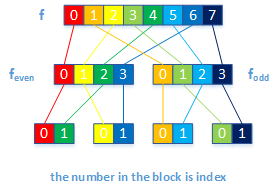
\includegraphics[width=0.4\textwidth]{assets/FFT.png}
\end{figure}